\documentclass{standalone}
\usepackage{tikz}
\usetikzlibrary{patterns, positioning}
\usepackage[sfdefault]{ClearSans} %% option 'sfdefault' activates Clear Sans as the default text font
\usepackage[T1]{fontenc}

\begin{document}
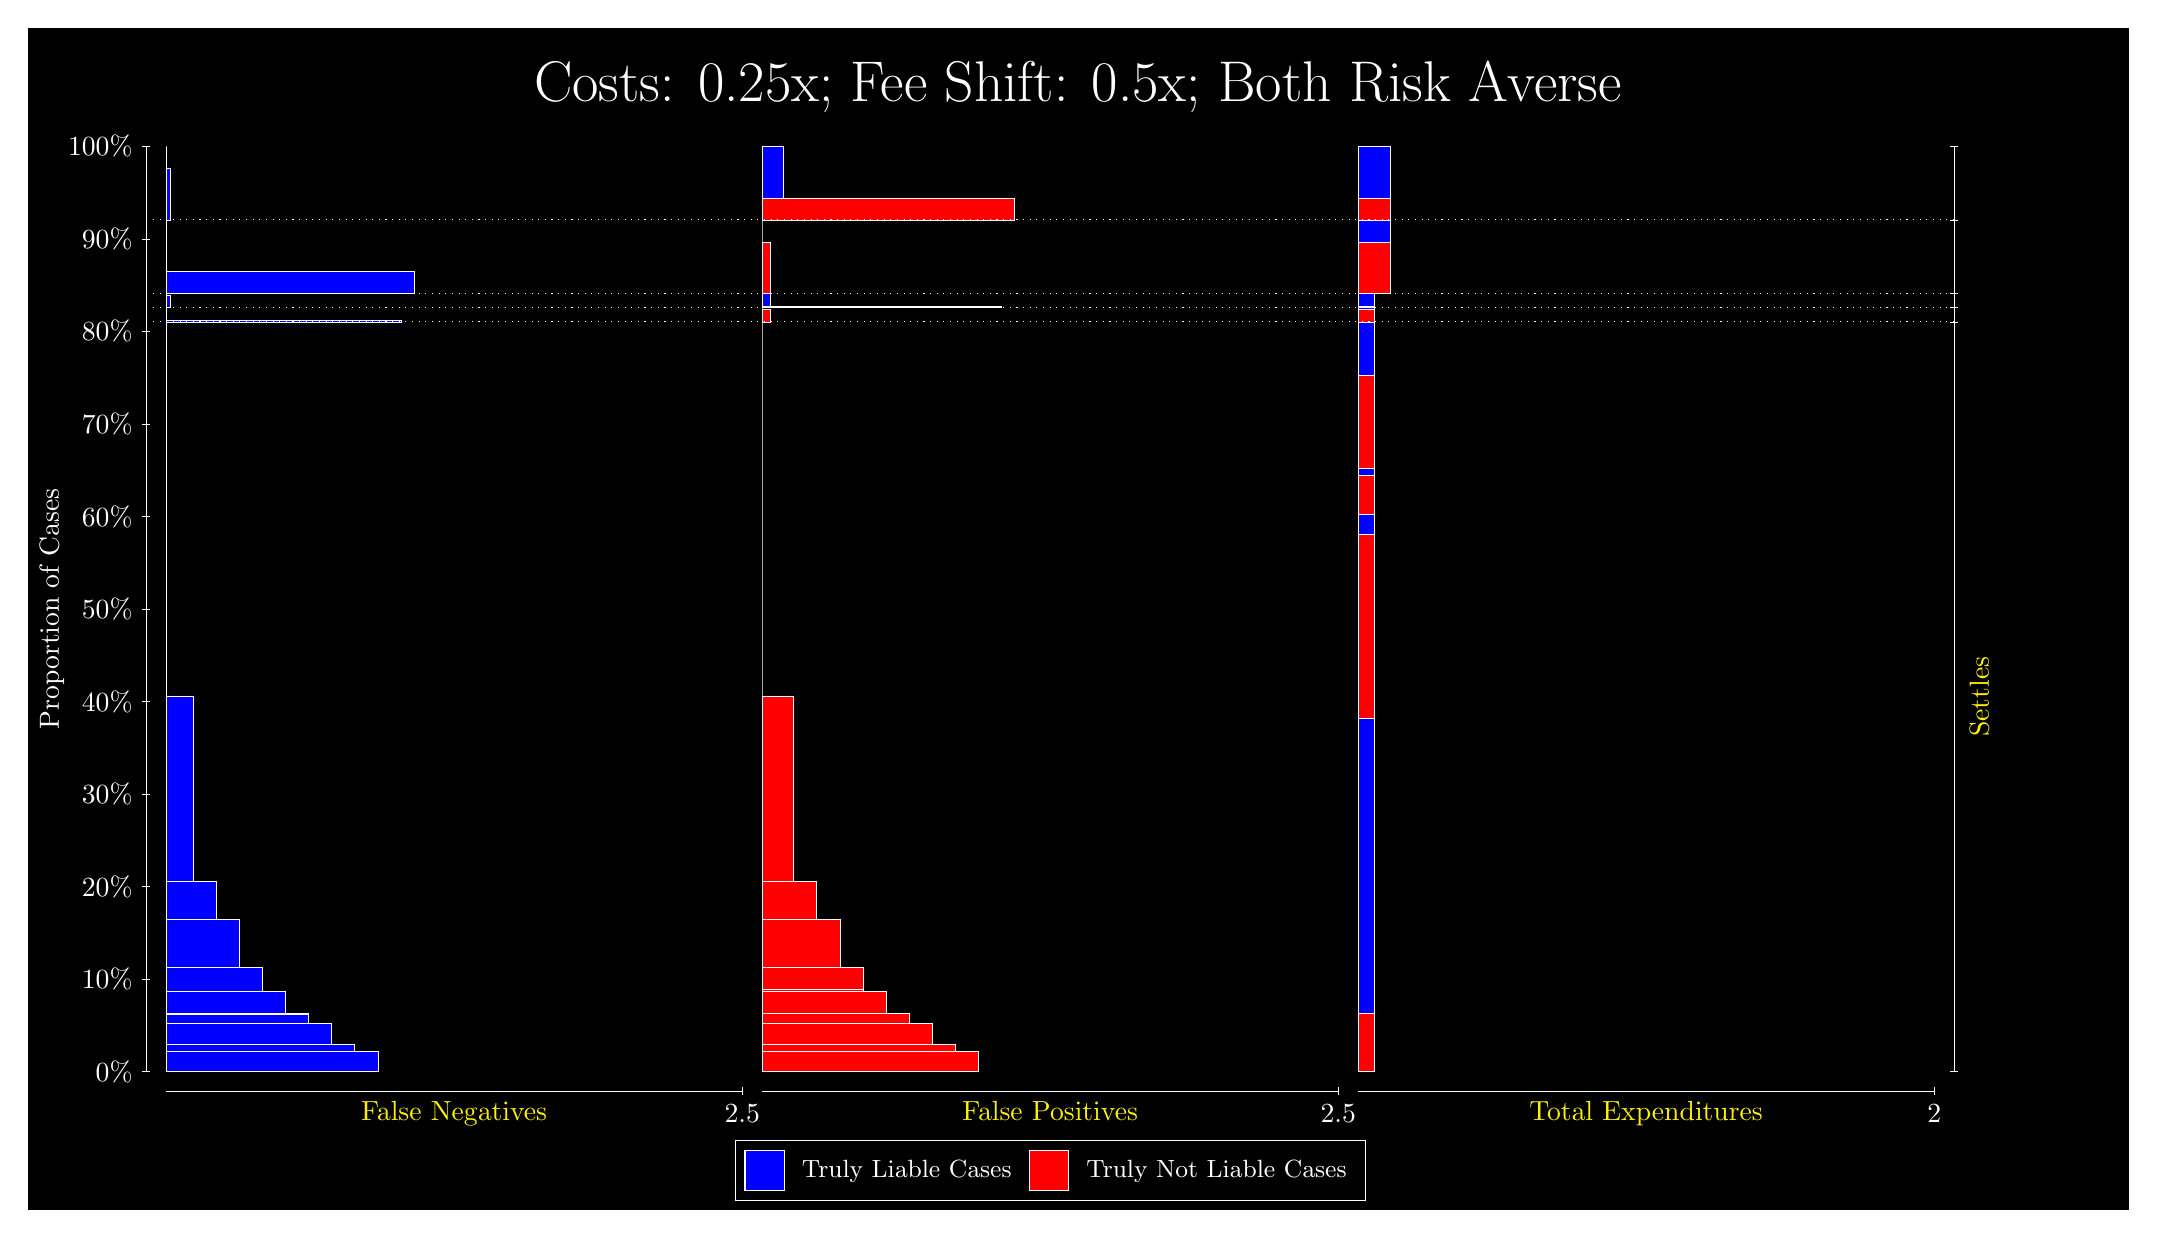
\begin{tikzpicture}
\draw[fill=black] (0,0) rectangle (26.667,15);
\draw[text=white] (0,13.5) rectangle (26.667,15) node[midway] {\huge Costs: 0.25x; Fee Shift: 0.5x; Both Risk Averse};
\draw[white, very thin] (1.5,1.75) -- (1.5,13.5);
\node[rotate=90, text=white, anchor=center] at (0.3, 7.625) {Proportion of Cases};
\draw[white, very thin] (1.45,1.75) -- (1.55,1.75);
\node[text=white, anchor=east] at (1.45, 1.75) {0\%};
\draw[white, very thin] (1.45,2.925) -- (1.55,2.925);
\node[text=white, anchor=east] at (1.45, 2.925) {10\%};
\draw[white, very thin] (1.45,4.1) -- (1.55,4.1);
\node[text=white, anchor=east] at (1.45, 4.1) {20\%};
\draw[white, very thin] (1.45,5.275) -- (1.55,5.275);
\node[text=white, anchor=east] at (1.45, 5.275) {30\%};
\draw[white, very thin] (1.45,6.45) -- (1.55,6.45);
\node[text=white, anchor=east] at (1.45, 6.45) {40\%};
\draw[white, very thin] (1.45,7.625) -- (1.55,7.625);
\node[text=white, anchor=east] at (1.45, 7.625) {50\%};
\draw[white, very thin] (1.45,8.8) -- (1.55,8.8);
\node[text=white, anchor=east] at (1.45, 8.8) {60\%};
\draw[white, very thin] (1.45,9.975) -- (1.55,9.975);
\node[text=white, anchor=east] at (1.45, 9.975) {70\%};
\draw[white, very thin] (1.45,11.15) -- (1.55,11.15);
\node[text=white, anchor=east] at (1.45, 11.15) {80\%};
\draw[white, very thin] (1.45,12.325) -- (1.55,12.325);
\node[text=white, anchor=east] at (1.45, 12.325) {90\%};
\draw[white, very thin] (1.45,13.5) -- (1.55,13.5);
\node[text=white, anchor=east] at (1.45, 13.5) {100\%};

\draw[white, very thin] (24.457,1.75) -- (24.457,13.5);
\draw[white, very thin] (24.407,1.75) -- (24.507,1.75);
\node[anchor=west] at (24.407, 1.75) {};
\draw[white, very thin] (24.407,11.271) -- (24.507,11.271);
\node[anchor=west] at (24.407, 11.271) {};
\draw[white, very thin] (24.407,11.45) -- (24.507,11.45);
\node[anchor=west] at (24.407, 11.45) {};
\draw[white, very thin] (24.407,11.629) -- (24.507,11.629);
\node[anchor=west] at (24.407, 11.629) {};
\draw[white, very thin] (24.407,12.565) -- (24.507,12.565);
\node[anchor=west] at (24.407, 12.565) {};
\draw[white, very thin] (24.407,13.5) -- (24.507,13.5);
\node[anchor=west] at (24.407, 13.5) {};

\draw[white, very thin, fill=blue] (1.75,1.75) rectangle (4.4397,2.0079);
\draw[white, very thin, fill=blue] (1.75,2.0079) rectangle (4.1469,2.0908);
\draw[white, very thin, fill=blue] (1.75,2.0908) rectangle (3.8542,2.3568);
\draw[white, very thin, fill=blue] (1.75,2.3568) rectangle (3.5614,2.4743);
\draw[white, very thin, fill=blue] (1.75,2.4743) rectangle (3.5614,2.494);
\draw[white, very thin, fill=blue] (1.75,2.494) rectangle (3.2687,2.7697);
\draw[white, very thin, fill=blue] (1.75,2.7697) rectangle (2.9759,3.0767);
\draw[white, very thin, fill=blue] (1.75,3.0767) rectangle (2.6832,3.6773);
\draw[white, very thin, fill=blue] (1.75,3.6773) rectangle (2.3904,4.1713);
\draw[white, very thin, fill=blue] (1.75,4.1713) rectangle (2.0976,6.5106);
\draw[white, very thin, fill=red] (1.75,6.5106) rectangle (1.75,11.271);
\draw[white, very thin, fill=blue] (1.75,11.271) rectangle (4.7324,11.291);
\draw[white, very thin, fill=red] (1.75,11.291) rectangle (1.75,11.45);
\draw[white, very thin, fill=blue] (1.75,11.45) rectangle (1.8049,11.61);
\draw[white, very thin, fill=red] (1.75,11.61) rectangle (1.75,11.629);
\draw[white, very thin, fill=blue] (1.75,11.629) rectangle (4.8971,11.908);
\draw[white, very thin, fill=red] (1.75,11.908) rectangle (1.75,12.565);
\draw[white, very thin, fill=blue] (1.75,12.565) rectangle (1.8049,13.222);
\draw[white, very thin, fill=red] (1.75,13.222) rectangle (1.75,13.5);
\draw[white, very thin, fill=red] (9.3189,1.75) rectangle (12.063,2.0079);
\draw[white, very thin, fill=red] (9.3189,2.0079) rectangle (11.771,2.0908);
\draw[white, very thin, fill=red] (9.3189,2.0908) rectangle (11.478,2.3568);
\draw[white, very thin, fill=red] (9.3189,2.3568) rectangle (11.185,2.4939);
\draw[white, very thin, fill=red] (9.3189,2.4939) rectangle (10.892,2.7697);
\draw[white, very thin, fill=red] (9.3189,2.7697) rectangle (10.6,2.7893);
\draw[white, very thin, fill=red] (9.3189,2.7893) rectangle (10.6,3.0766);
\draw[white, very thin, fill=red] (9.3189,3.0766) rectangle (10.307,3.6773);
\draw[white, very thin, fill=red] (9.3189,3.6773) rectangle (10.014,4.1714);
\draw[white, very thin, fill=red] (9.3189,4.1714) rectangle (9.7214,6.5107);
\draw[white, very thin, fill=blue] (9.3189,6.5107) rectangle (9.3189,11.271);
\draw[white, very thin, fill=red] (9.3189,11.271) rectangle (9.4287,11.431);
\draw[white, very thin, fill=blue] (9.3189,11.431) rectangle (9.3189,11.45);
\draw[white, very thin, fill=red] (9.3189,11.45) rectangle (12.356,11.47);
\draw[white, very thin, fill=blue] (9.3189,11.47) rectangle (9.4287,11.629);
\draw[white, very thin, fill=red] (9.3189,11.629) rectangle (9.4287,12.286);
\draw[white, very thin, fill=blue] (9.3189,12.286) rectangle (9.3189,12.565);
\draw[white, very thin, fill=red] (9.3189,12.565) rectangle (12.521,12.843);
\draw[white, very thin, fill=blue] (9.3189,12.843) rectangle (9.5933,13.5);
\draw[white, very thin, fill=red] (16.888,1.75) rectangle (17.094,2.4939);
\draw[white, very thin, fill=blue] (16.888,2.4939) rectangle (17.094,6.2348);
\draw[white, very thin, fill=red] (16.888,6.2348) rectangle (17.094,8.5741);
\draw[white, very thin, fill=blue] (16.888,8.5741) rectangle (17.094,8.8321);
\draw[white, very thin, fill=red] (16.888,8.8321) rectangle (17.094,9.3262);
\draw[white, very thin, fill=blue] (16.888,9.3262) rectangle (17.094,9.4091);
\draw[white, very thin, fill=red] (16.888,9.4091) rectangle (17.094,10.592);
\draw[white, very thin, fill=blue] (16.888,10.592) rectangle (17.094,11.271);
\draw[white, very thin, fill=red] (16.888,11.271) rectangle (17.094,11.431);
\draw[white, very thin, fill=blue] (16.888,11.431) rectangle (17.094,11.45);
\draw[white, very thin, fill=red] (16.888,11.45) rectangle (17.094,11.47);
\draw[white, very thin, fill=blue] (16.888,11.47) rectangle (17.094,11.629);
\draw[white, very thin, fill=red] (16.888,11.629) rectangle (17.299,12.286);
\draw[white, very thin, fill=blue] (16.888,12.286) rectangle (17.299,12.565);
\draw[white, very thin, fill=red] (16.888,12.565) rectangle (17.299,12.843);
\draw[white, very thin, fill=blue] (16.888,12.843) rectangle (17.299,13.5);
\draw[white, dotted] (1.5,11.271) -- (24.457,11.271);
\draw[white, dotted] (1.5,11.45) -- (24.457,11.45);
\draw[white, dotted] (1.5,11.629) -- (24.457,11.629);
\draw[white, dotted] (1.5,12.565) -- (24.457,12.565);
\draw[white, very thin] (1.75,1.5) -- (9.0689,1.5);
\node[text=yellow, anchor=north] at (5.4094, 1.5) {False Negatives};
\draw[white, very thin] (9.0689,1.45) -- (9.0689,1.55);
\node[text=white, anchor=north] at (9.0689, 1.45) {2.5};

\draw[white, very thin] (9.3189,1.5) -- (16.638,1.5);
\node[text=yellow, anchor=north] at (12.978, 1.5) {False Positives};
\draw[white, very thin] (16.638,1.45) -- (16.638,1.55);
\node[text=white, anchor=north] at (16.638, 1.45) {2.5};

\draw[white, very thin] (16.888,1.5) -- (24.207,1.5);
\node[text=yellow, anchor=north] at (20.547, 1.5) {Total Expenditures};
\draw[white, very thin] (24.207,1.45) -- (24.207,1.55);
\node[text=white, anchor=north] at (24.207, 1.45) {2};

\node[text=yellow, centered, rotate=90] at (24.777, 6.5106) {Settles};





\draw (12.978300999999998,1.5) node[draw=none] (baseCoordinate) {};
\begin{scope}[align=center]
        \matrix[scale=0.5, draw=white, below=0.5cm of baseCoordinate, nodes={draw}, column sep=0.1cm]{
            \node[rectangle, draw, minimum width=0.5cm, minimum height=0.5cm, fill=blue] {}; &
            \node[draw=none, font=\small, text=white] (B) {Truly Liable Cases}; &
            \node[rectangle, draw, minimum width=0.5cm, minimum height=0.5cm, fill=red] {}; &
            \node[draw=none, font=\small, text=white] (B) {Truly Not Liable Cases}; \\
            };
\end{scope}

\end{tikzpicture}
\end{document}